% Reproducible TikZ renderer for Figure 7. All layout values are in centimetres.
\documentclass[tikz,border=2pt]{standalone}
\usepackage[T1]{fontenc}
\usetikzlibrary{arrows.meta,calc,positioning}
\renewcommand\familydefault{\sfdefault}
\definecolor{sourcefill}{HTML}{DDEBF7}
\definecolor{trainfill}{HTML}{FCE4D6}
\definecolor{runtimefill}{HTML}{E2F0D9}
\definecolor{systemfill}{HTML}{EDE7F6}
\definecolor{loopfill}{HTML}{FFF2CC}
\definecolor{edgegray}{HTML}{5F6B76}
\definecolor{bordergray}{HTML}{71808C}
\definecolor{textgray}{HTML}{3B4650}
\definecolor{subtext}{HTML}{5D6871}
\newcommand{\mechanismtext}{\fontsize{7.25}{8.4}\selectfont\color{subtext}}
\newcommand{\reptext}{\fontsize{6.4}{7.4}\selectfont\color{subtext}}
\newcommand{\methodtext}{\fontsize{7.15}{8.3}\selectfont\color{textgray}}

\tikzset{
  >={Stealth[length=2.2mm,width=1.5mm]},
  flow/.style={->,draw=edgegray,line width=.55pt},
  feedback/.style={->,draw=edgegray,line width=.7pt},
  mainbox/.style={draw=bordergray,line width=.6pt,rounded corners=2.3pt,align=center,text=textgray,inner sep=3.5pt},
  groupbox/.style={draw=bordergray!65,line width=.48pt,rounded corners=3.0pt,fill=white},
  branch/.style={mainbox,minimum width=3.48cm,minimum height=2.1cm},
  tiny/.style={font=\fontsize{6.4}{7.4}\selectfont,text=subtext},
  mechanism/.style={font=\fontsize{7.25}{8.4}\selectfont,text=subtext},
  methods/.style={font=\fontsize{7.15}{8.3}\selectfont,text=textgray},
  smallbox/.style={draw=bordergray,line width=.45pt,rounded corners=1.7pt,align=center,inner sep=2.5pt,font=\fontsize{6.85}{7.8}\selectfont,text=textgray}
}

\begin{document}
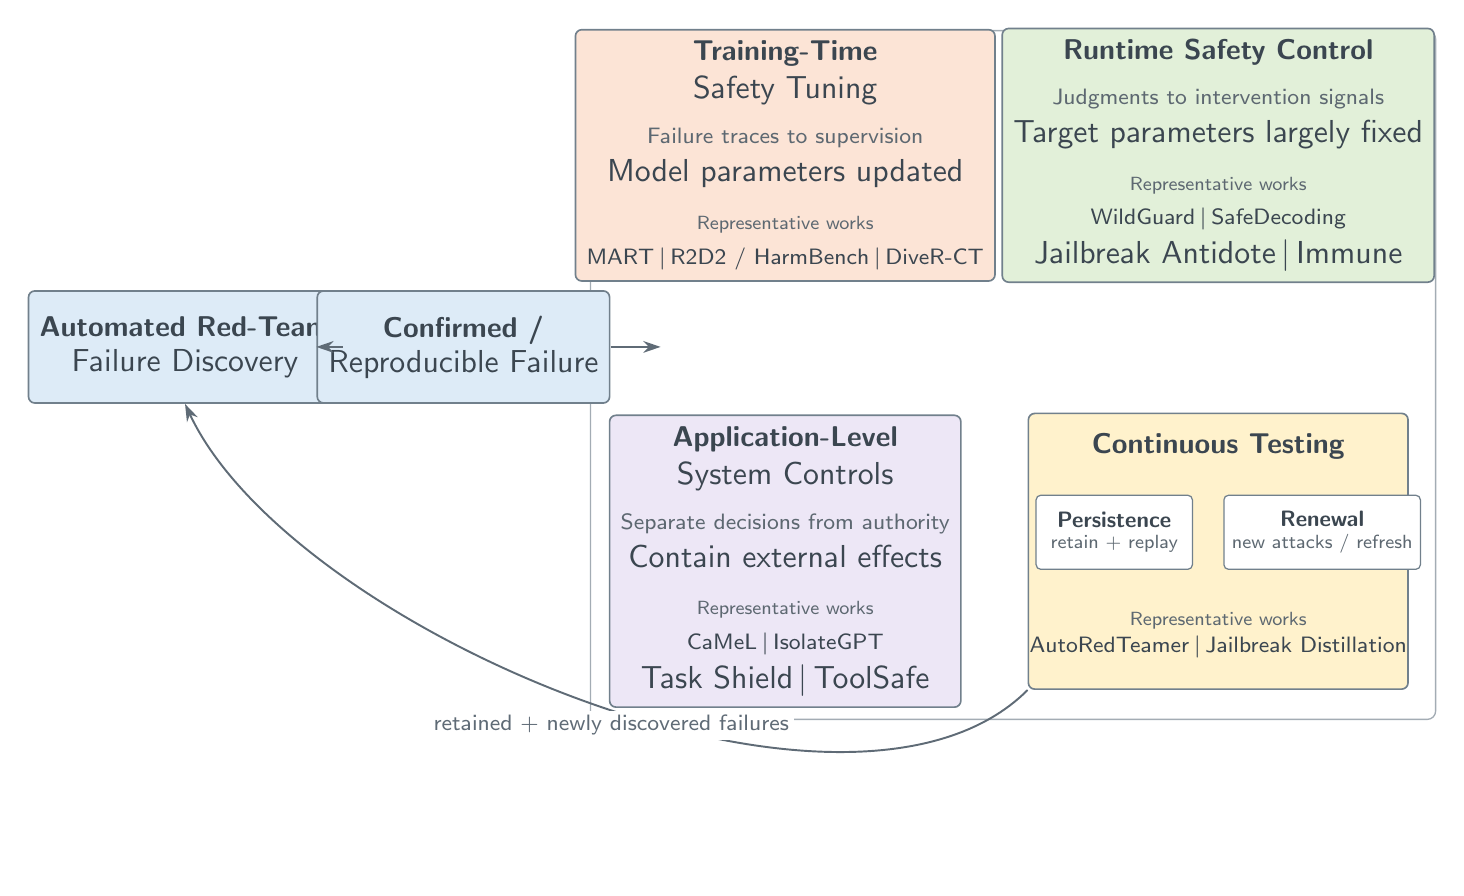
\begin{tikzpicture}[x=1cm,y=1cm,scale=1.148,transform shape]
  % Draw the taxonomy frame first so source nodes remain unobscured.
  \node[groupbox,minimum width=9.35cm,minimum height=7.62cm] (reusepanel) at (10.78,3.99) {};
  \coordinate (reuseentry) at (6.88,4.30);

  % Source and decision nodes.
  \node[mainbox,fill=sourcefill,minimum width=2.48cm,minimum height=1.24cm] (discovery) at (1.62,4.30) {\bfseries\fontsize{9.1}{10.2}\selectfont Automated Red-Team\\[-1pt]Failure Discovery};
  \node[mainbox,fill=sourcefill,minimum width=2.57cm,minimum height=1.24cm] (confirmed) at (4.70,4.30) {\bfseries\fontsize{9.1}{10.2}\selectfont Confirmed /\\[-1pt]Reproducible Failure};

  % Four remediation branches.
  \node[branch,fill=trainfill] (training) at (8.26,6.42) {\bfseries\fontsize{9.2}{10.3}\selectfont Training-Time\\Safety Tuning\\[2.1pt]\mechanismtext Failure traces to supervision\\Model parameters updated\\[3pt]\reptext Representative works\\[-1pt]\methodtext MART\hspace{.18em}\textbar\hspace{.18em}R2D2 / HarmBench\hspace{.18em}\textbar\hspace{.18em}DiveR-CT};

  \node[branch,fill=runtimefill,minimum width=3.82cm] (runtime) at (13.05,6.42) {\bfseries\fontsize{9.2}{10.3}\selectfont Runtime Safety Control\\[2.1pt]\mechanismtext Judgments to intervention signals\\Target parameters largely fixed\\[3pt]\reptext Representative works\\[-1pt]\methodtext WildGuard\hspace{.18em}\textbar\hspace{.18em}SafeDecoding\\Jailbreak Antidote\hspace{.18em}\textbar\hspace{.18em}Immune};

  \node[branch,fill=systemfill] (system) at (8.26,1.93) {\bfseries\fontsize{9.2}{10.3}\selectfont Application-Level\\System Controls\\[2.1pt]\mechanismtext Separate decisions from authority\\Contain external effects\\[3pt]\reptext Representative works\\[-1pt]\methodtext CaMeL\hspace{.18em}\textbar\hspace{.18em}IsolateGPT\\Task Shield\hspace{.18em}\textbar\hspace{.18em}ToolSafe};

  \node[mainbox,fill=loopfill,minimum width=4.20cm,minimum height=3.05cm] (continuous) at (13.05,2.04) {};
  \node[font=\bfseries\fontsize{9.2}{10.3}\selectfont,text=textgray] at (13.05,3.20) {Continuous Testing};
  \node[smallbox,fill=white,minimum width=1.73cm,minimum height=.82cm] (persistence) at (11.90,2.25) {\bfseries Persistence\\[-1pt]\reptext retain + replay};
  \node[smallbox,fill=white,minimum width=1.73cm,minimum height=.82cm] (renewal) at (14.20,2.25) {\bfseries Renewal\\[-1pt]\reptext new attacks / refresh};
  \node[tiny] at (13.05,1.27) {\strut Representative works};
  \node[methods] at (13.05,.98) {\methodtext AutoRedTeamer\hspace{.18em}\textbar\hspace{.18em}Jailbreak Distillation};

  % The confirmed case enters a four-level remediation taxonomy.
  \draw[flow] (discovery.east) -- (confirmed.west);
  \draw[flow] (confirmed.east) -- (reuseentry);

  % The feedback edge explicitly closes the red-teaming loop.
  \draw[feedback] (continuous.south west) to[out=225,in=-65,looseness=.72] node[below,font=\fontsize{7.15}{8}\selectfont,text=edgegray,pos=.47,fill=white,inner sep=1.5pt] {retained + newly discovered failures} (discovery.south);
\end{tikzpicture}
\end{document}
